\documentclass[english]{tktltiki}
\usepackage[pdftex]{graphicx}
\usepackage{subfigure}
\usepackage{url}
\usepackage{tabularx}
\usepackage{booktabs}
\begin{document}
\onehalfspacing

\title{Location Awareness - Project work: Scratch Off Map}
\author{P�ter Ivanics}
\date{\today}

\maketitle

\numberofpagesinformation{\numberofpages\ pages + \numberofappendixpages\ appendices}
\keywords{}

\mytableofcontents

\section{Introduction}
	This report is a summary of my project work for the Location Awareness course, which is a simple location-based game called Scratch-Off Map for iOS devices. The high level idea of the game is to provide a place for users to show which countries they visited so far. For instance, once a user enters a new country where he has not been to before, the application would recognize that based on the location and mark the country as visited. 
	
	The identification of the visited countries works based on GIS coordinates and their reverse geocoding to country names. As the users collect more and more coordinates by time, the list of points and therefore the list of visited countries grow as they travel around the world. 
	
	To utilize techniques learned throughout the course, the collection of points can be scheduled according to a Duty Cycling mechanism. Using this technique way the network traffic, reverse-geocoding queries and the battery life can be considerably reduced. 
	
	The measured points can be visualized and the visited countries can be colored on the world map. Based on the measured points in individual countries, the colors may differ and the user may be presented a leaderboard of his/her most visited countries. The user may want to create a "wish-list" of countries to visit next, that are also shown on the visual map with different color than the visited ones. 
	
	To achieve the data collection, reverse geocoding feature, the visualization of the map and the points, the API of Apple's MapKit \footnote{\url{https://developer.apple.com/reference/mapkit}} framework is utilized. My personal motivation behind choosing this project is to
	
	\begin{itemize}
		\item gain hands-on experience in the field of Location Awareness,
		\item implement Duty Cycling and potentially other techniques covered during the course inside the application,
		\item learn the usage and the APIs of the MapKit framework as a specimen of a locationing-oriented framework,
		\item improve my skills in iOS and Swift 3.0 development, Test Driven Development (TDD), Object-Oriented Programming (OOP), mobile databases and in technical writing,
		\item further explore the field of Location Awareness. 
	\end{itemize}

\section{Development plans}
	To begin the development with, the development plans are carried out, platform, development language and tools are chosen. First, the feature list of the application are stated in Table \ref{feature-list}. Naturally, the features which create the core of the software such as data collection, duty cycling, reverse-geocoding and basic data visualization are put on on higher priority (1) than other features, which may enhance the user experience, but not essential to demonstrate gains of the Location Awareness course. Therefore such features are marked as lower priority (3) and some of them are not even part of the final, working application.
	
	\begin{table}[]
\caption{The planned features, their explanations and priority (1 = high priority, 3 = low priority) for the Scratch Off Map. }
\label{feature-list}
\begin{tabularx}{\textwidth}{ l p{3.3cm} X p{.1cm}}
\toprule
\# & \textbf{Feature}                                              & \textbf{Explanation}                                                                                                                                                                                                                                                                                             & \textbf{Priority} \\ \midrule
\textbf{1}  & \textbf{Duty Cycling}                                                  & The collection of data points should run according to a Duty Cycling schedule. The user should be able to modify this schedule as (s)he likes, for instance by choosing between 1/3/5/10 minute cycles or by inserting values manually.                                                                          & 1                 \\ \hline
\textbf{2}  & \textbf{Force new data point collection}                               & The user should be able to manually initiate collection of a new longitude-latitude coordinate pair where (s)he is at currently.                                                                                                                                                                                 & 1                 \\ \hline
\textbf{3}  & \textbf{Manual data point insertion}                                   & The user should be able to manually insert a longitude-latitude coordinate pair and add it to the database.                                                                                                                                                                                                      & 3                 \\ \hline
\textbf{4}  & \textbf{List of visited countries}                                     & The user should be able to display the list of countries (s)he visited so far based on the collected points in the database.                                                                                                                                                                                     & 1                 \\ \hline
\textbf{5}  & \textbf{Number of points from individual countries}                    & The user should see how many points from each country (s)he collected.                                                                                                                                                                                                                                           & 2                 \\ \hline
\textbf{6}  & \textbf{Reverse-geocoding of coordinates to country names {[}codes{]}} & The application should be able to reverse the longitude-latitude coordinate pairs and tell the country to which the coordinates belong to. For instance, input (60.1699, 24.9384) would give the result of Finland {[}FI{]}.                                                                                     & 1                 \\ \hline
\textbf{7}  & \textbf{Visualization of visited countries on the world map}           & The application should be able to color the visited countries on the world map. The color of the countries may differ based on the number of the points that were identified to be in that country (for instance countries with many points have dark, countries with small number of points have light colors). & 3                 \\ \hline
\textbf{8}  & \textbf{Visualization of the collected points on the world map}        & The application should be able to visualize the collected points on the world map (for instance, by putting pins or points at the coordinates and displaying them on the screen).                                                                                                                                & 2                 \\ \hline
\textbf{9}  & \textbf{"Scratch-off" new countries}                                   & Once a new country is visited, the user should be able to "scratch-off" the new country from the map. The map of the country is displayed in a full-screen view and the user can scratch/swipe the dust off from the country to make it visited (as on scratch-off lottery tickets).                             & 4                 \\ \bottomrule
\end{tabularx}
\end{table}
	
	The development target for the application are iOS 10.0-ready mobile devices. More specifically, this includes iPhones and iPads (mobile phone and tablet devices). The integrated developer environment (IDE) is chosen to be xCode 8.2.1 \footnote{\url{https://itunes.apple.com/fi/app/xcode/id497799835?mt=12}}, while the programming language is Swift 3.0 \footnote{\url{https://developer.apple.com/library/content/documentation/Swift/Conceptual/Swift_Programming_Language/}}.  On top of that, the project is put under version control (git) so the development process and debugging can be fluent and more efficient. The reason behind choosing this platform, developer environment, tools and programming language is their popularity, my personal interest and familiarity with them. 
	
	For development approach, Test Driven Development (TDD) is chosen, at least for the application's business logic layer. The reason behind this decision is the fact that it is simple to implement and strongly contributes to software quality and easy maintainability \cite{clean-coder}. 

\subsection{Architectural overview}

To understand how the software works, the architectural design is explained shortly in this chapter. This includes the main components, UML (Unified Modeling Language) diagrams and their brief explanation. Activity and detailed diagrams are excluded from this report due to its small scope.

The applications main design pattern follows the Model View Controller (MVC) approach in general. However, as suggested by several professionals (\cite{orl15}, \cite{per16}), this particular design has the risk of going into the Massive View Controller direction in case of iOS development and is not recommended. As the scope of this project for the time being is limited, other design patterns are not discussed nor included in the development. Nevertheless, this finding is kept in mind and the views of the application are kept minimal and the business logic is separated in different components as explained in the paragraphs to follow.

The component diagram of the Scratch Off Map is displayed on Figure \ref{compontent-diagram}. The application's Model components at this point is very simple as it has only two classes: $Coordinates$ and $Country$. These classes formulate the tables of the database and the objects that will store the user data during the application's execution.

The DatabaseManager class is part of the business logic and is responsible to serve as an interface between the main application Lifecycle Controller and the models. This component (which is actually reduced to a single class for now) is the main responsible for handling the business logic interacting with other components. On top of the data manipulation this means the maintenance of the CoordinateCollector and the GeoCoder services. The latter two service is also considered as an interfaces to the end-points of the MapKit library provided by Apple (using the Adapter pattern \footnote{\url{https://en.wikipedia.org/wiki/Adapter_pattern}}). The DatabaseManager component is designed exactly in the same manner to the end-points of the RealmSwift mobile database \footnote{\url{https://realm.io/}}, which is a community-build open source library. 

Finally, the UIViewController classes represent the data that is retrieved through the LifecycleManager. As pointed out above, the logic in these classes is kept minimal and focused only on user interface-related issues. These classes also utilize the capabilities of the built-in MapKit and UIKit packages. 

\begin{figure}[h]
\ \newline
\begin{center}
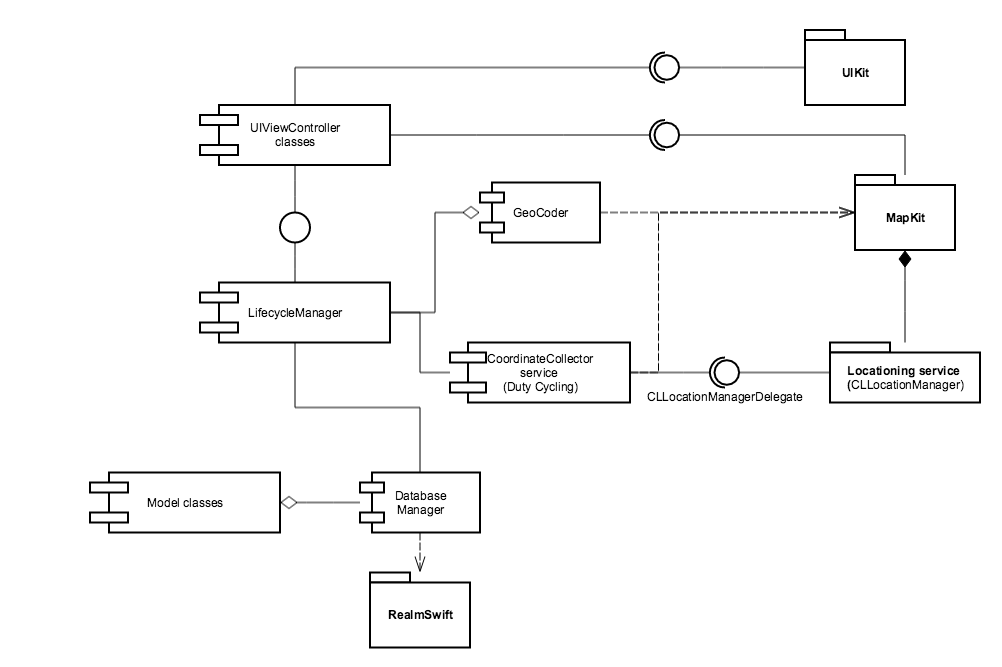
\includegraphics[width=0.9\textwidth]{images/ScratchOffMap-component_diagram.png}
\caption{The component diagram of the Scratch Off Map application.}
\label{component-diagram}
\end{center}
\end{figure}

\subsection{Implementation steps and challenges}
After planning the features and the software architecture, the implementation of the software began. A Github repository \footnote{\url{https://github.com/ivanicspeter92/ScratchOffMap}} was created for the version tracking of the source code. Next, the Xcode project was set up and configured, including the test project. Next, the project structure was established to include the following folders to help understanding : 

	\begin{enumerate}
		\item Controllers
		\item Extensions
		\item Models
		\item Protocols
		\item Storyboards
		\item Views
	\end{enumerate}

	\subsection{Models}	
	As the first step of the development, the model classes $Country$ and $Coordinates$ were developed and tested. The latter included some more complex logic such as instantiating coordinates from using strings, the $CoordinatesTests$ class includes a couple of automated tests for this functionality.
	
	The classes above are very primitive and have only a couple of fields and initializers. Any type of complex business logic is stored in the controller classes and is not handled in the models. Naturally, this is a very sophisticated and simple set of model objects due to the simplicity of the application, however the architecture is yet open for extensions and further addition of functionality. 
	
	\subsection{Controllers}
	Next, the $DutyCycling$ and its subclass, $CoordinateCollectorService$ was implemented. The former class is an abstract implementation of the duty cycling mechanism and designed in a way that it can be reused for other purposes. The latter is an extension of this functionality and performs the GIS data collection through the MapKit APIs. 
	
	\begin{figure}[h]
	\ \newline
	\begin{center}
	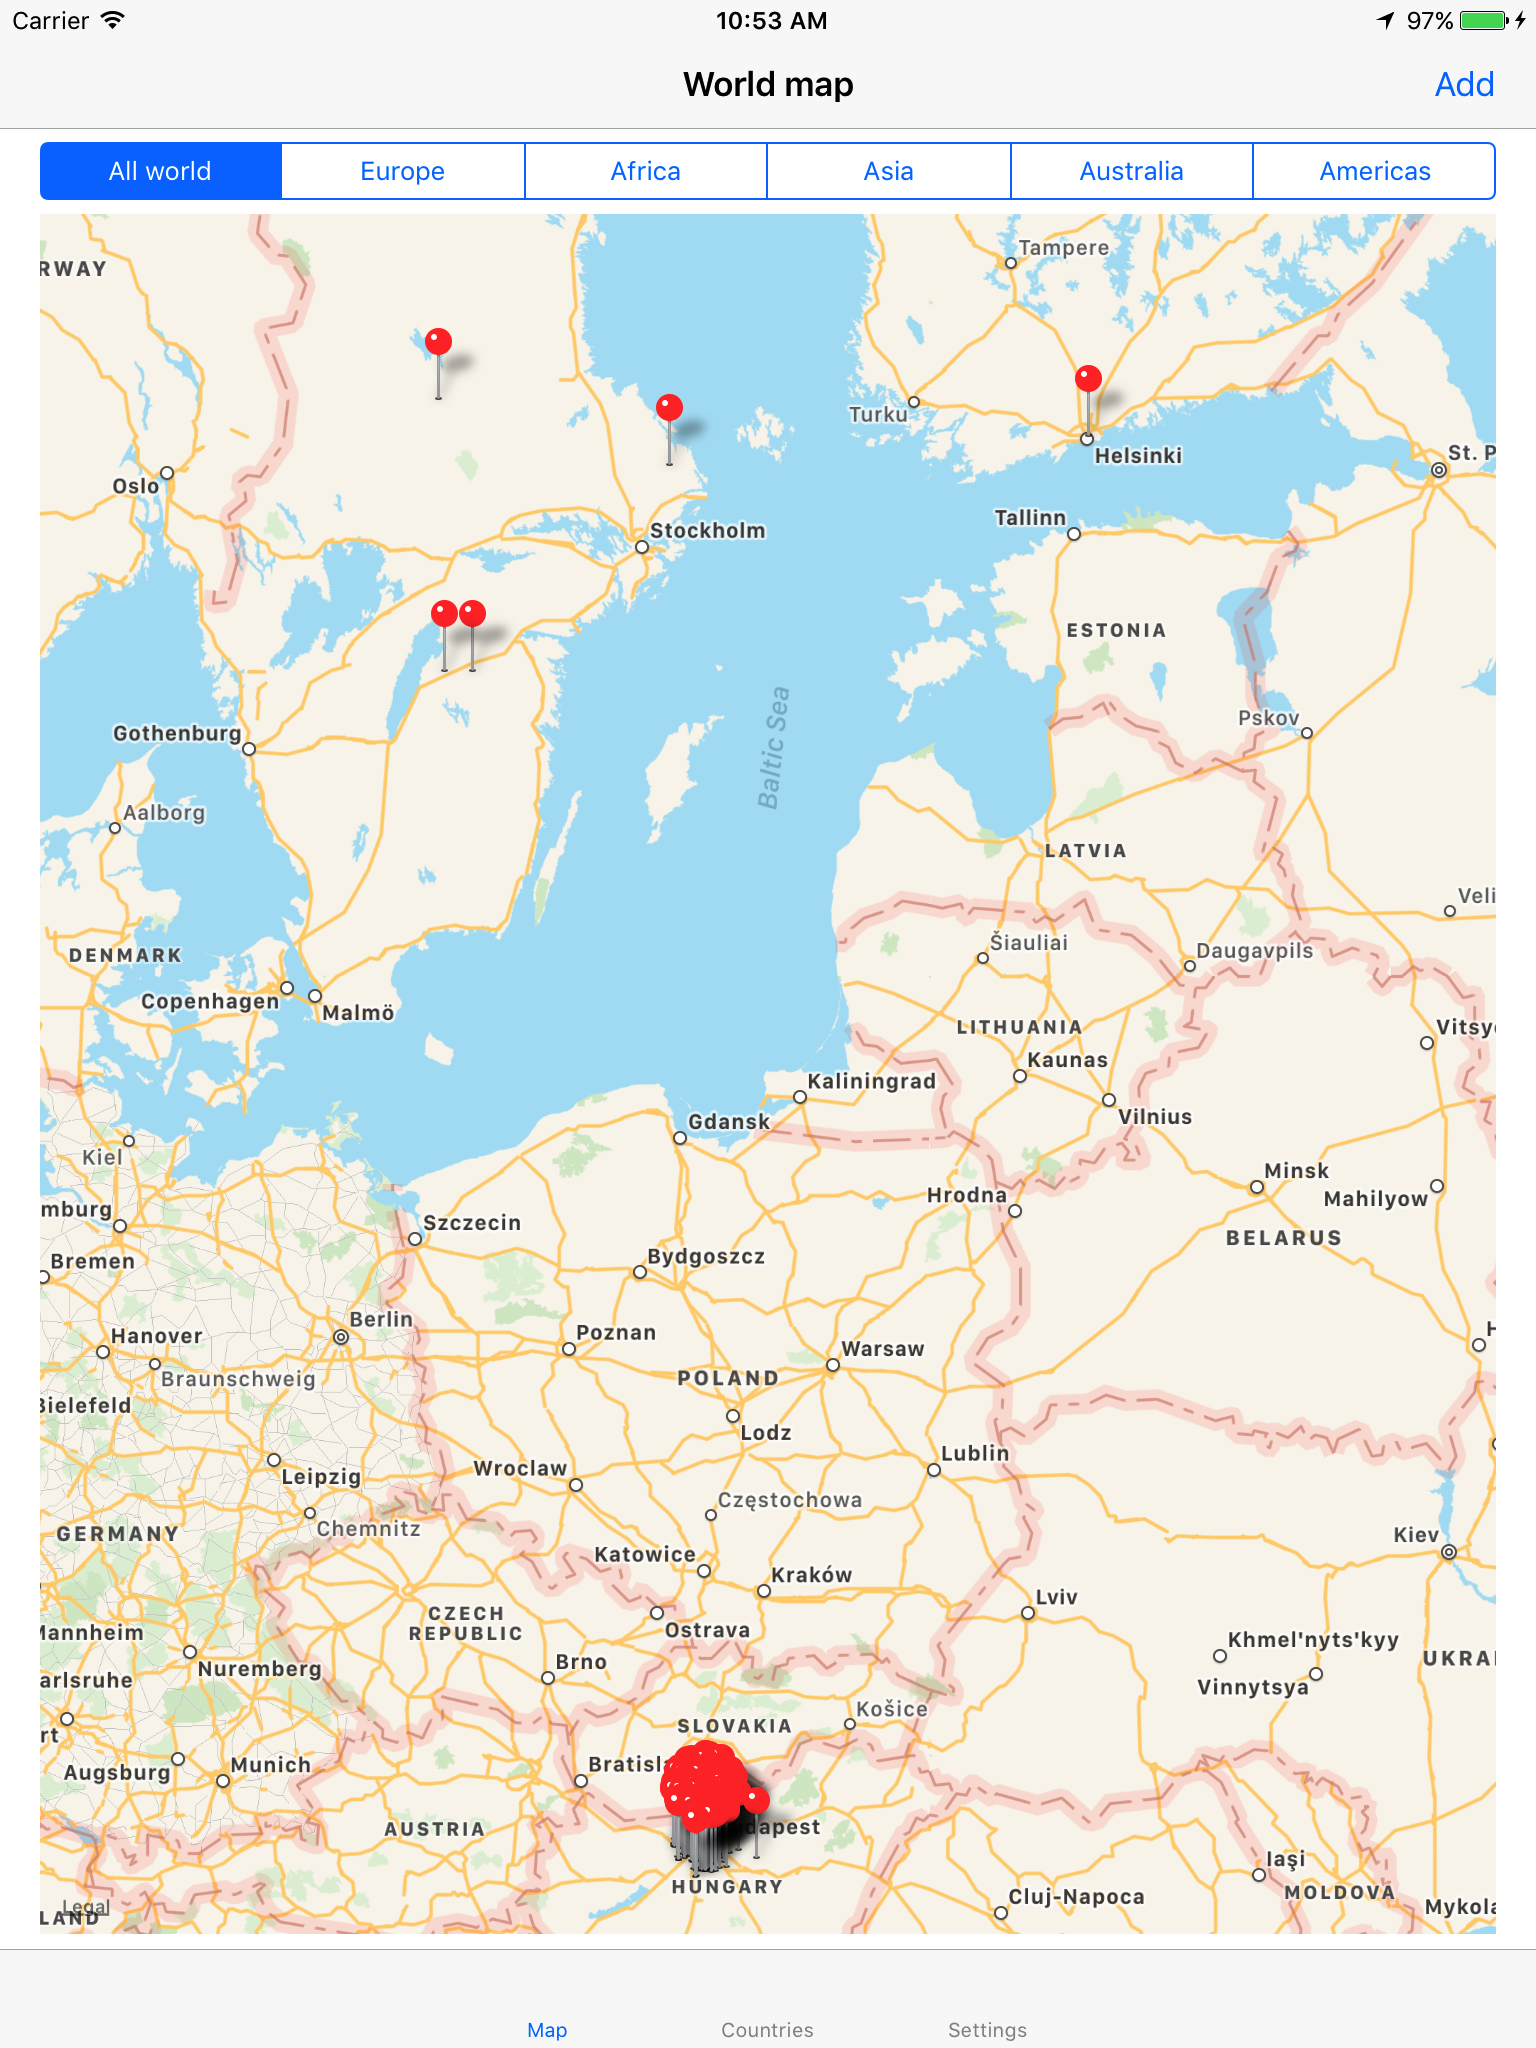
\includegraphics[width=0.4\textwidth]{images/points_in_europe.png}
	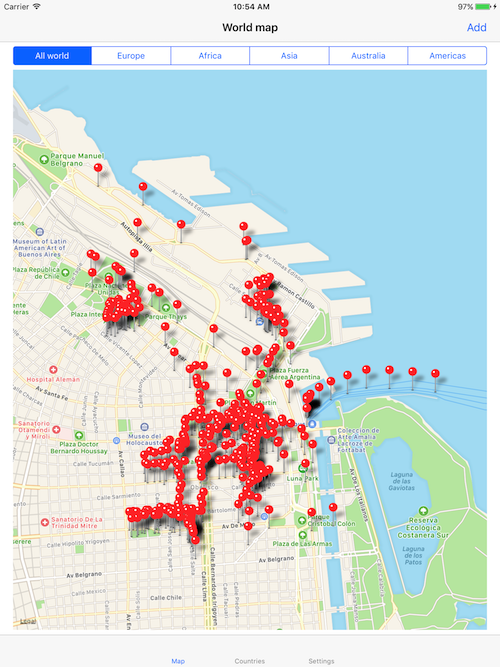
\includegraphics[width=0.4\textwidth]{images/buenos_aires.png}
	\caption{A set of points in Europe (left) and Argentina (right) visualized on the world map in the application.}
	\label{points_in_the_application}
	\end{center}
	\end{figure}	
	
	Afterwards, the $GeoCoder$ class was added and tested in $GeoCoderTests$. Integration with the API provided by MapKit was fairly straightforward, however I had to learn how to utilize closures and asynchronous testing to proceed with the efficient testing. I managed to get the reverse-geocoding working through the $decodeCountry()$ function of the $GeoCoder$ class. As the name suggests, this function is the main responsible for turning GPS coordinates and storing the unwrapped country to the database upon success. 
	
	During the testing it turned out that the reverse-geocoding service has the capability to retrieve more information than the country, for instance postal code, city or street name, if applicable. For this application, this data is dropped as only the country names were of interest. In some cases, typically while decoding high number of points, the API returned with an error message, which can be explained with the fact that the number of queries to the provider "are rate-limited for each app" according to the corresponding documentation \footnote{\url{https://developer.apple.com/reference/corelocation/clgeocoder/1423621-reversegeocodelocation}}. This problem was not resolved yet, because it appears only in a test environment, when huge set of points is added at once. In a real usage scenario the user collects only couple of points according to the duty cycle interval, and therefore the problem is not present.
	
	The country recognition in most cases is accurate, however in some cases the service recognized the country of the point to be an actual city (for instance in one case Hong Kong was returned as the country of a certain point). For this reason, such points are identified and hidden by default in the user interface. On top of that, the points that are collected without recognizing a country (e.g. if the point is in the middle of the ocean) are stored, but not presented to the user by default. The $DatabaseManager$ and the $LifecycleController$ is responsible jointly for handling such cases. 
	
	\subsection{Views}
	The user interface of the application contains three simple views: the world map, the list of visited countries and the application settings. As pointed out above, the corresponding classes ($WorldMapViewController, CountriesTableViewController$ and $SettingsTableViewController$) deal only with user interface-related issues and delegate all tasks to the controllers explained above. 
	
	\begin{figure}[h]
	\ \newline
	\begin{center}
	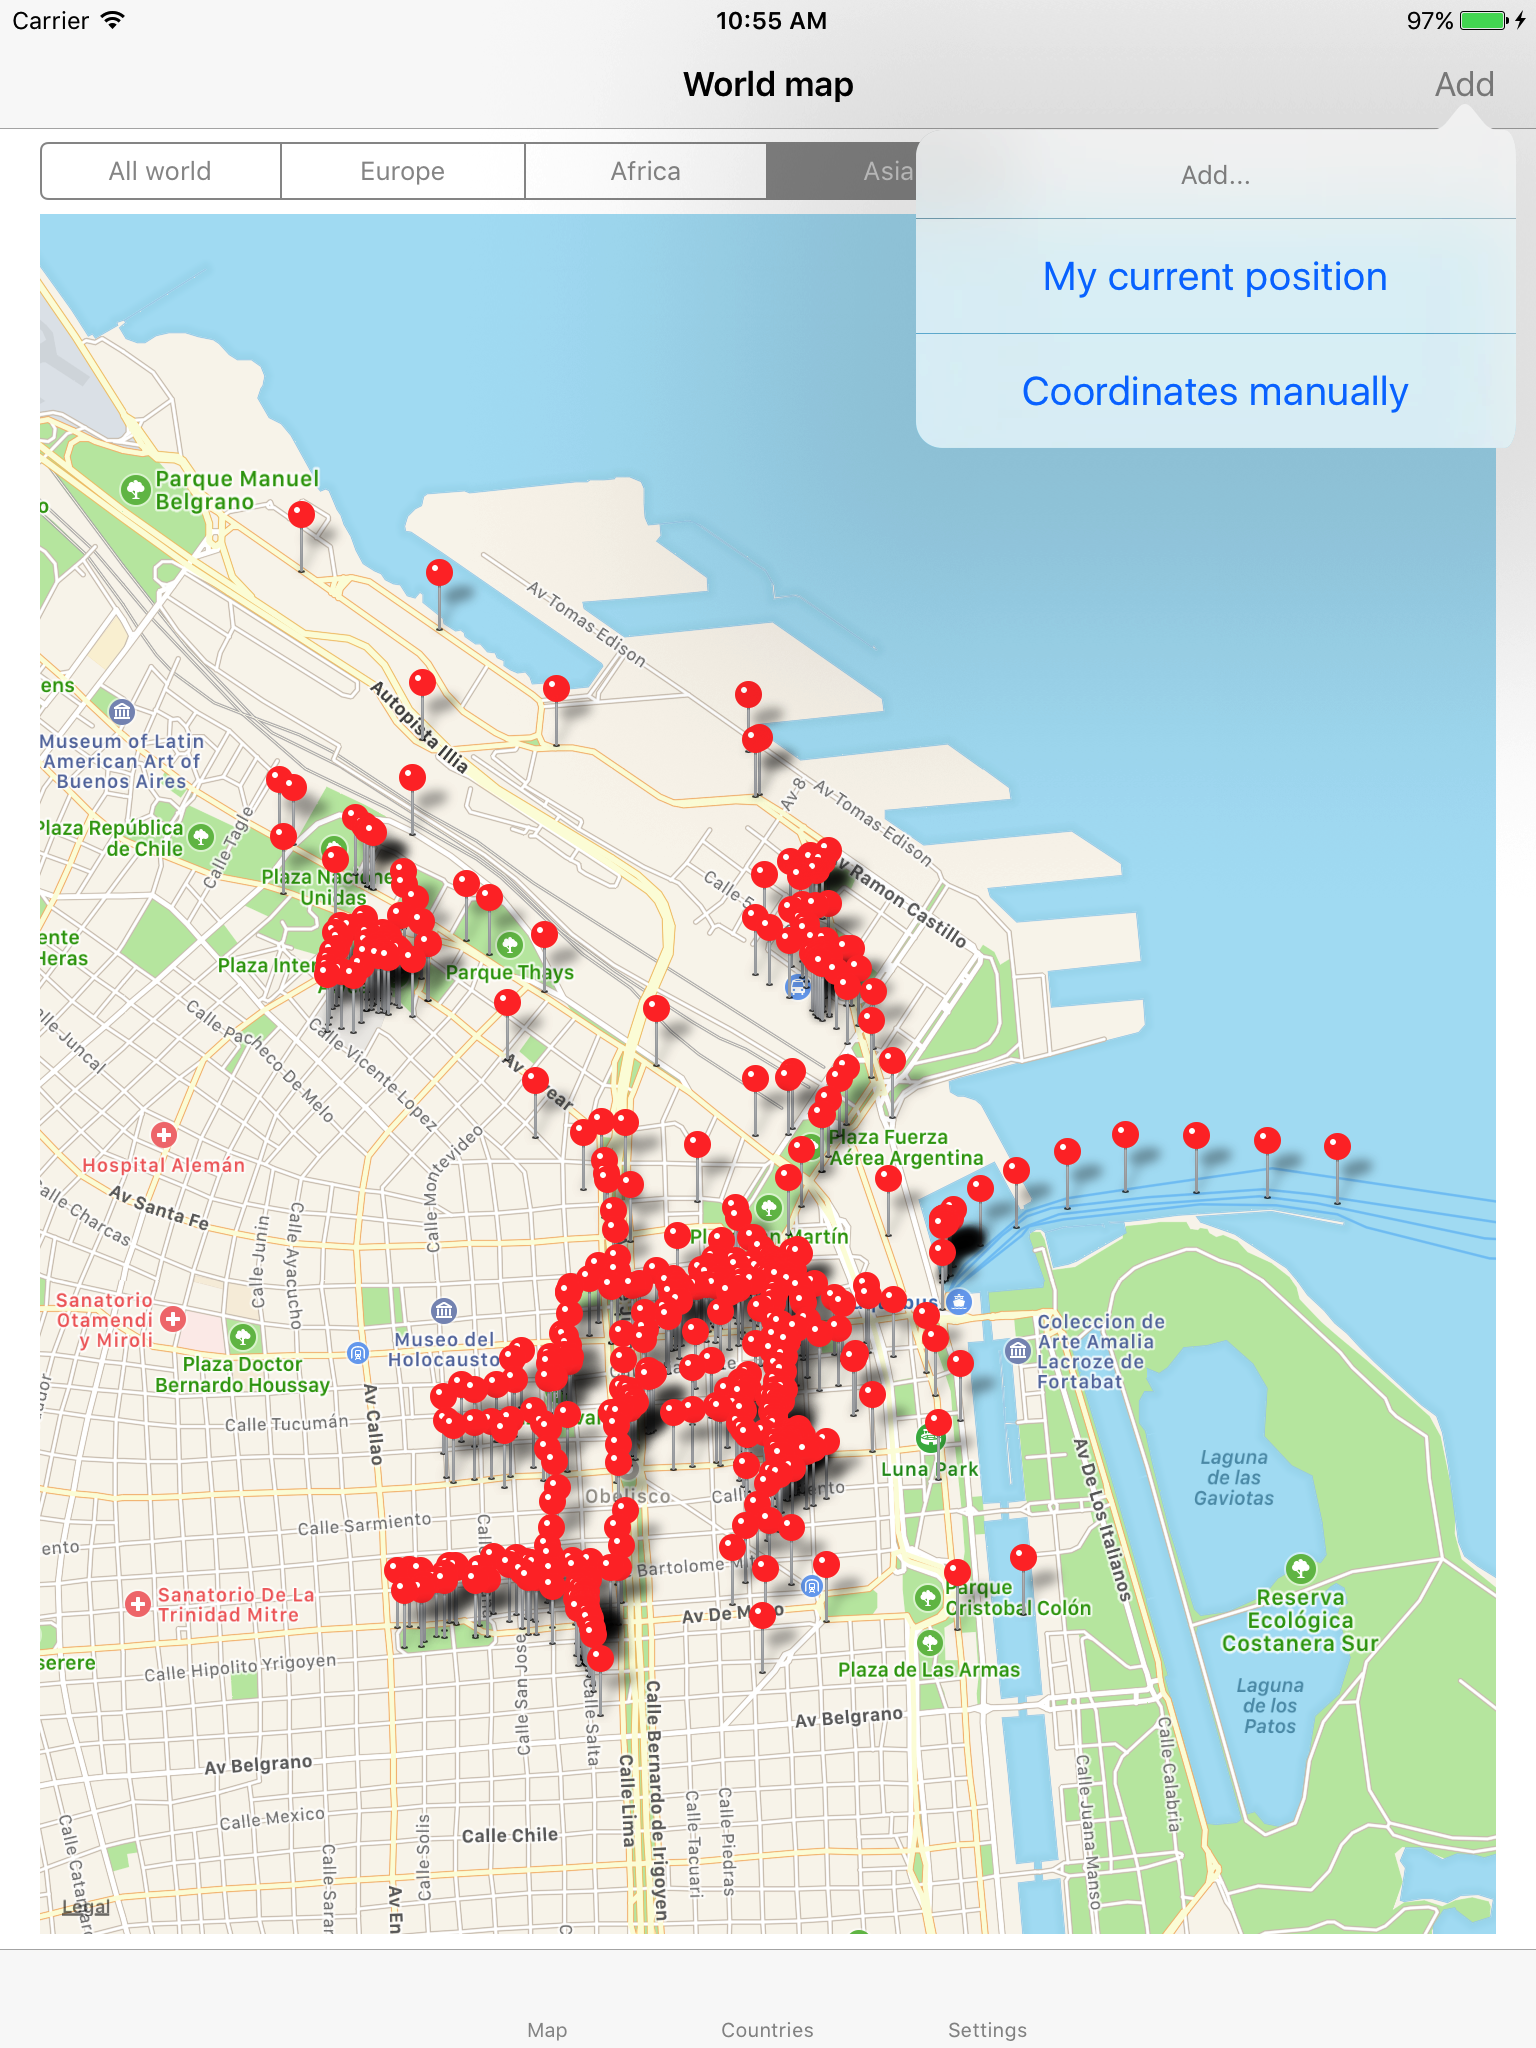
\includegraphics[width=0.4\textwidth]{images/point_addition.png}
	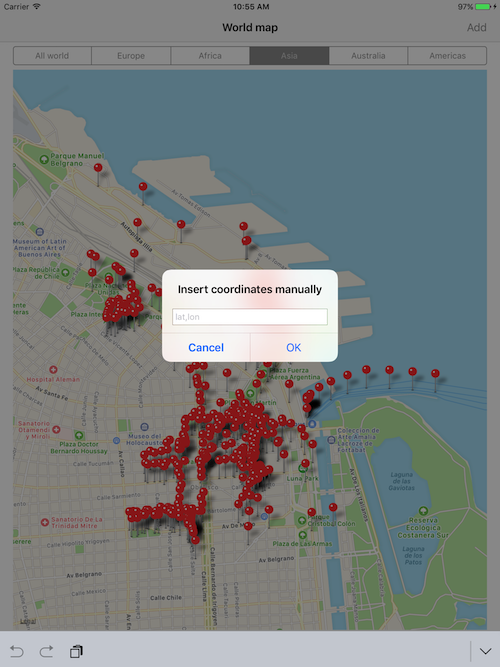
\includegraphics[width=0.4\textwidth]{images/manual_point_addition.png}
	\caption{Adding points by the current position of the device or by manual coordinate insertion.}
	\label{points_in_the_application}
	\end{center}
	\end{figure}		
	
	The $WorldMapViewController$ embeds a map (as an instance of the $MKMapView$ class), which displays the collected points on the map. For testing purposes I added several random points from Hungary, Sweden and Finland and a subset of the points in the Buenos Aires dataset to the database. The view successfully visualized these points on the map as shown of Figure \ref{points_in_the_application}. The view includes a "continent selector" control on the top of the screen. The idea of this control was to position the map above the selected continent, however this functionality was not added to the application yet. 
	
	By tapping on the "Add" button on the top-right corner of the screen the user may add new points to the database. This can be done either manually or by forcing the coordinate collector to trigger the duty cycle action - which is the retrieval of the current position of the device and storing the point into the database (Figure \ref{point_addition}). 

	Once the $GeoCoder$ service is enabled (through the $attemptDecodingCountriesInDatabase()$ function in the $LifecycleController$ class), the countries of the collected points are looked up and stored back in the database. Once a country is successfully recognized, it is displayed in list presented on the the $CountriesTableViewController$ as shown on Figure \ref{country_list}. Currently this view is limited to list the visited countries. Further improvement on this view could include displaying the number of points in each country on the right side, their clustering, analysis or statistics. 
	
	\begin{figure}[h]
	\ \newline
	\begin{center}
	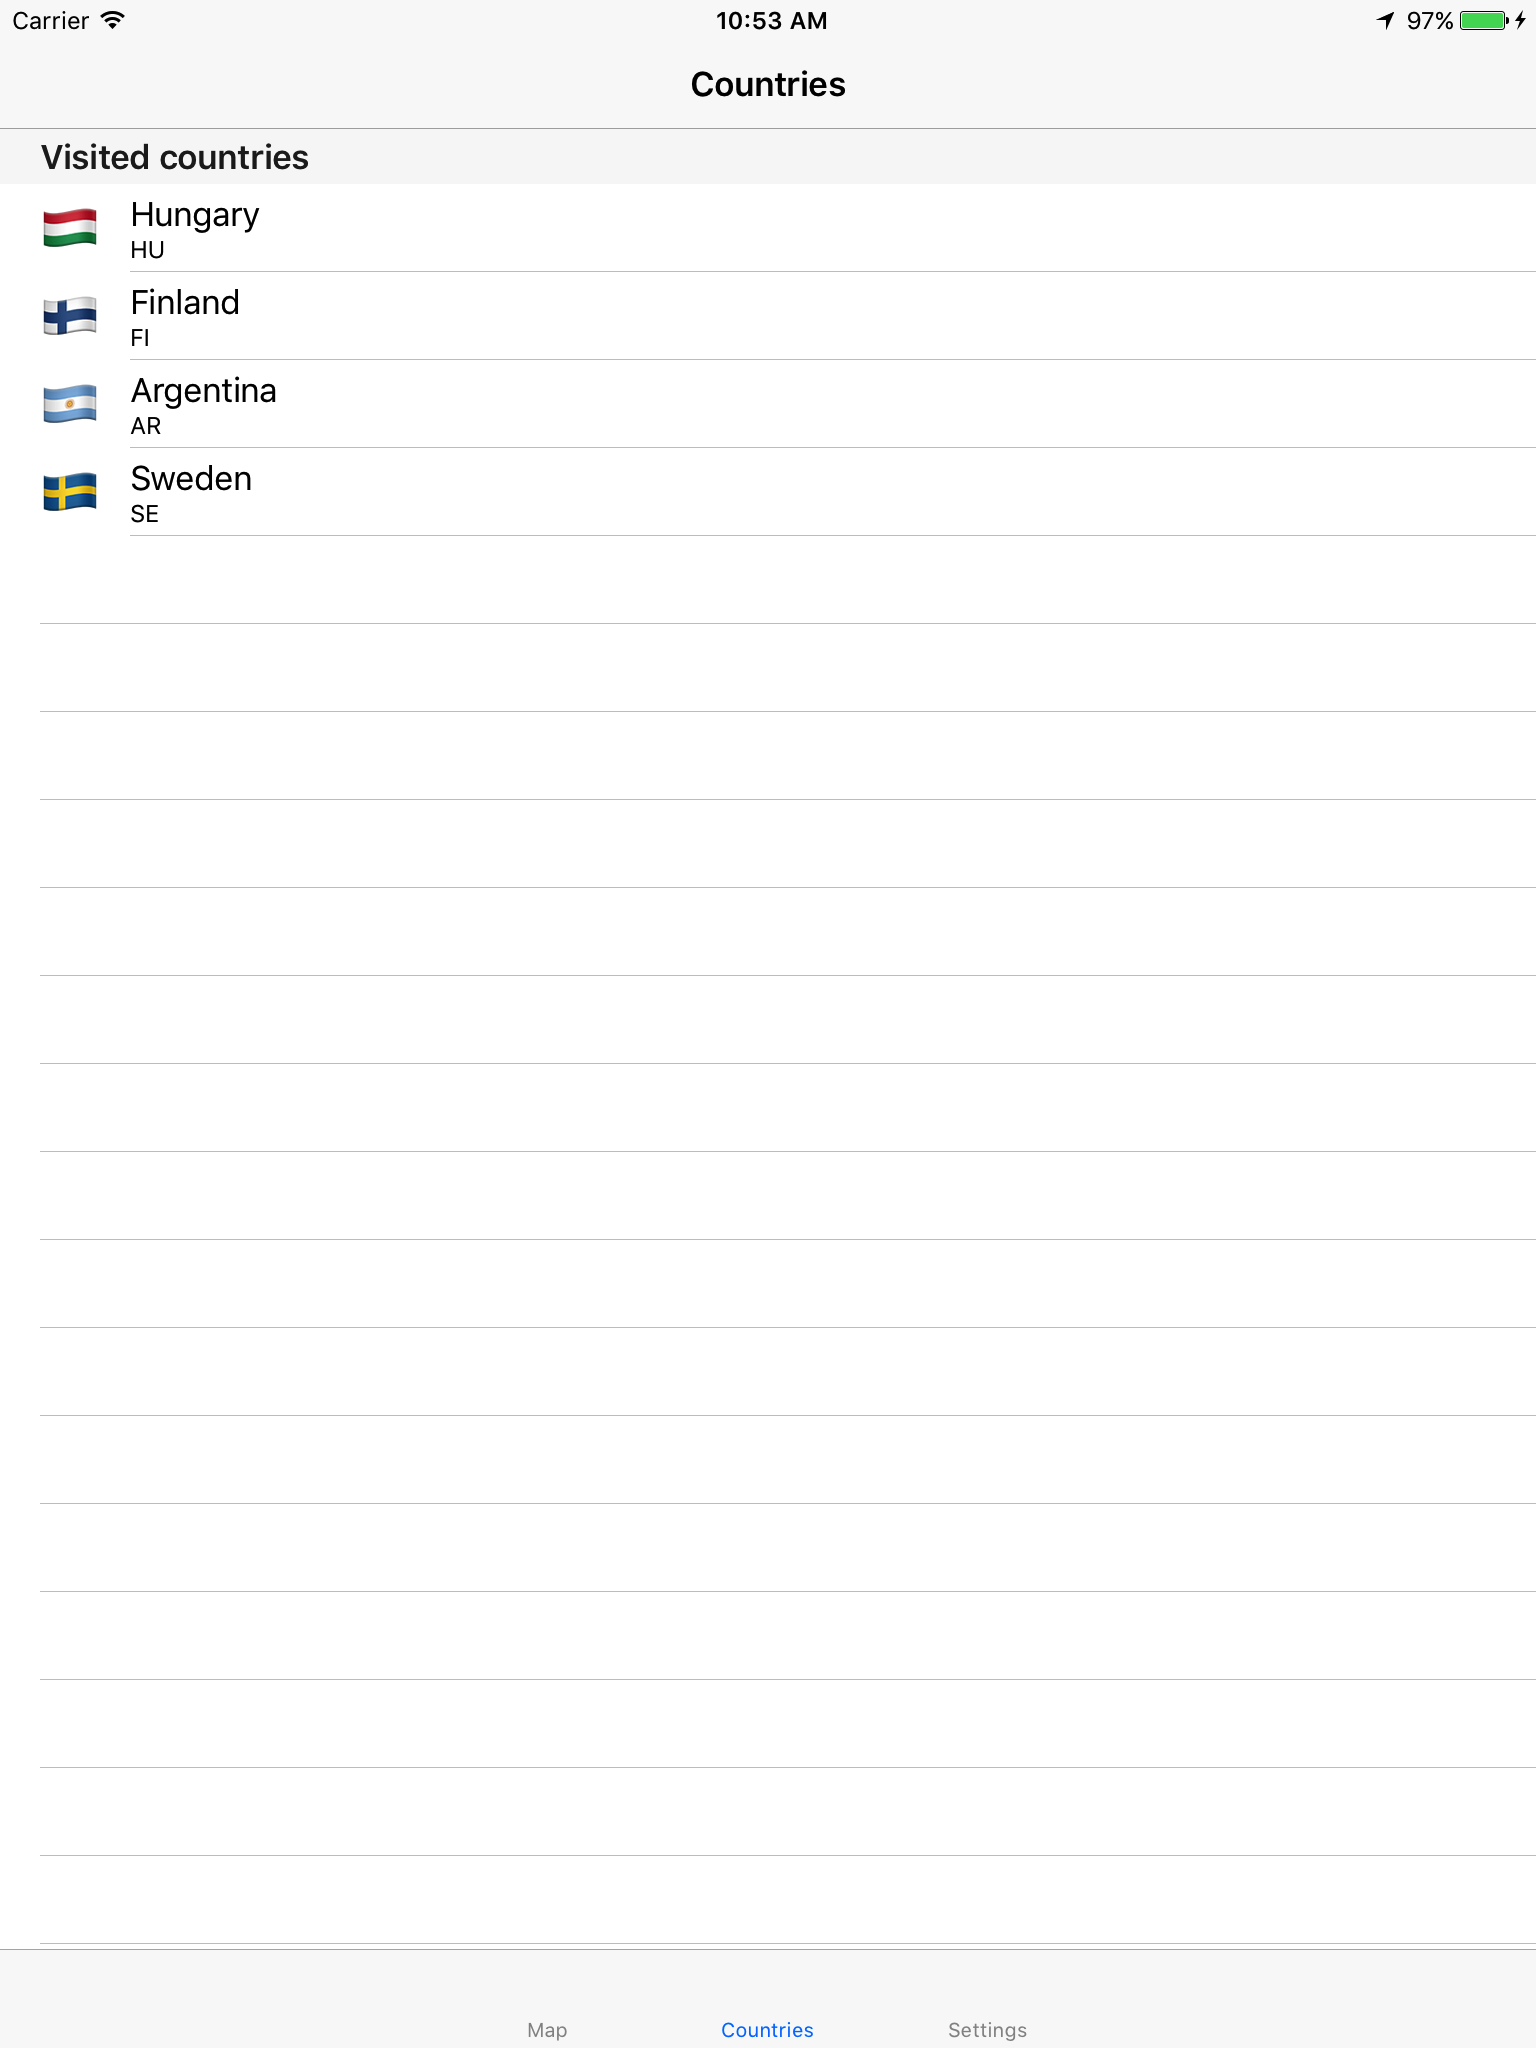
\includegraphics[width=0.4\textwidth]{images/country_list.png}
	\caption{The list of collected points. It is visible that the user currently has visited four countries: Hungary, Finland, Argentina and Sweden. }
	\label{country_list}
	\end{center}
	\end{figure}
	
	The $SettingsTableViewController$ provides a simple interface to manipulate the configuration of the application (Figure \ref{settings}). This includes changing the manipulation of the duty cycling interval (Figure \ref{modification_of_settings} left) of coordinate collection, displaying coordinates outside in the map, displaying countries without recognized country code in the list of visited countries and deletion of points from the database (Figure \ref{modification_of_settings} right). 

	\begin{figure}[h]
	\ \newline
	\begin{center}
	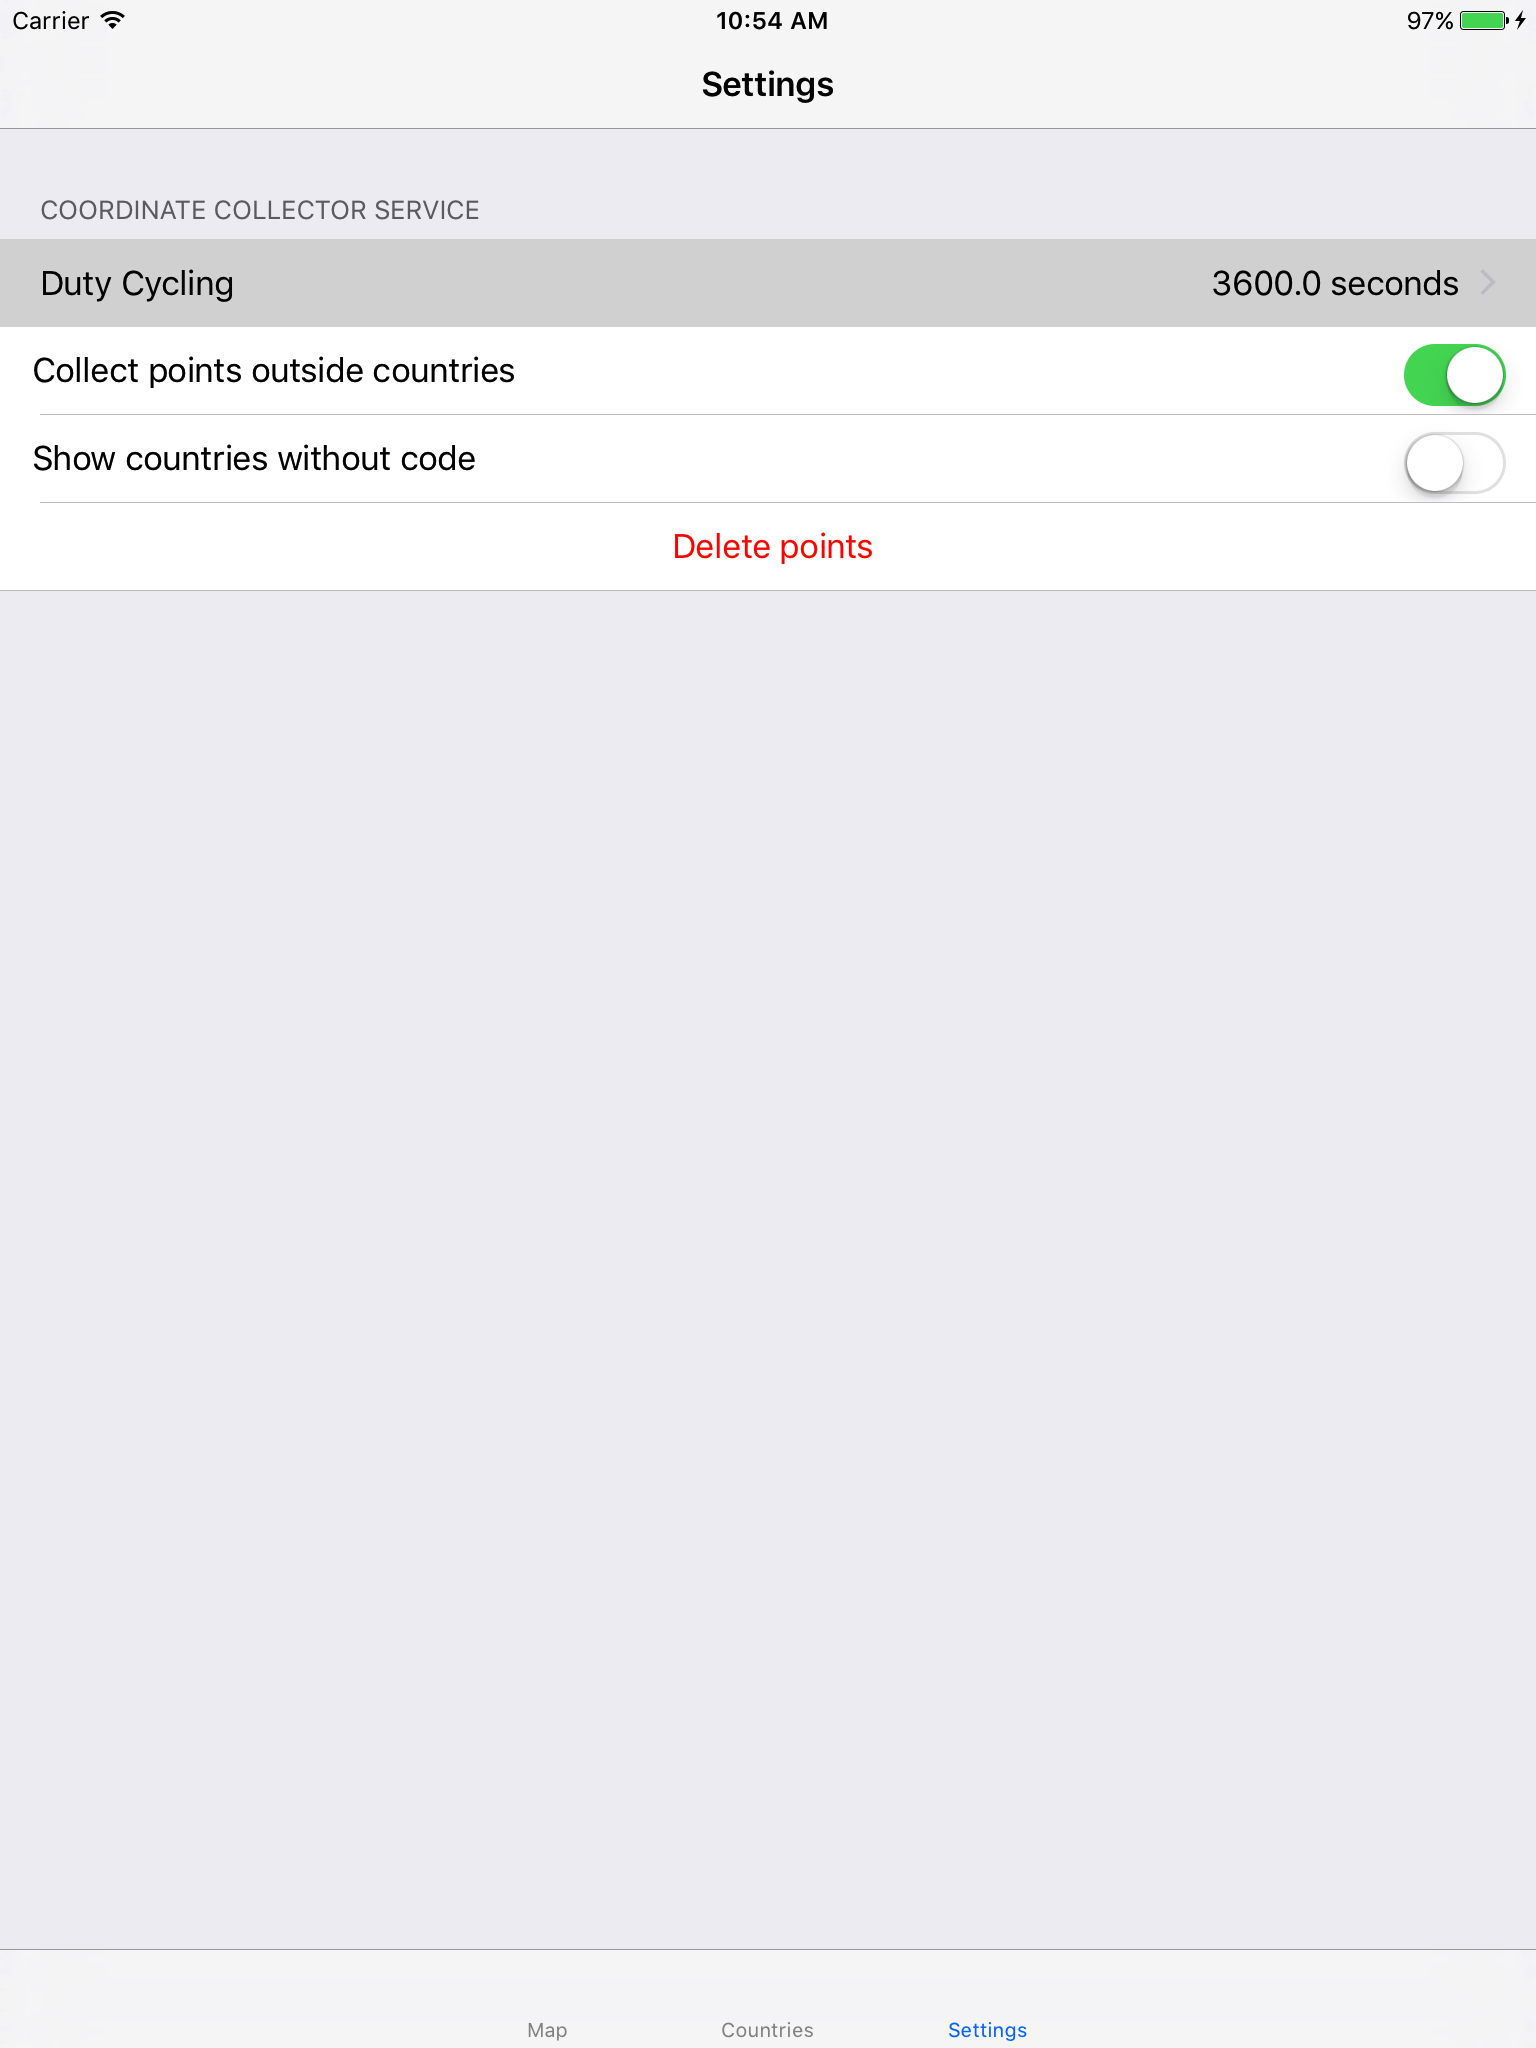
\includegraphics[width=0.4\textwidth]{images/settings.png}
	\caption{The settings view in the application.}
	\label{settings}
	\end{center}
	\end{figure}
	
	The settings are not stored to any temporal container and therefore are lost once the user exits the application. This feature was not part of the first iteration and therefore was not added, however it would be important and essential feature for further development.  

\begin{figure}[h]
	\ \newline
	\begin{center}
	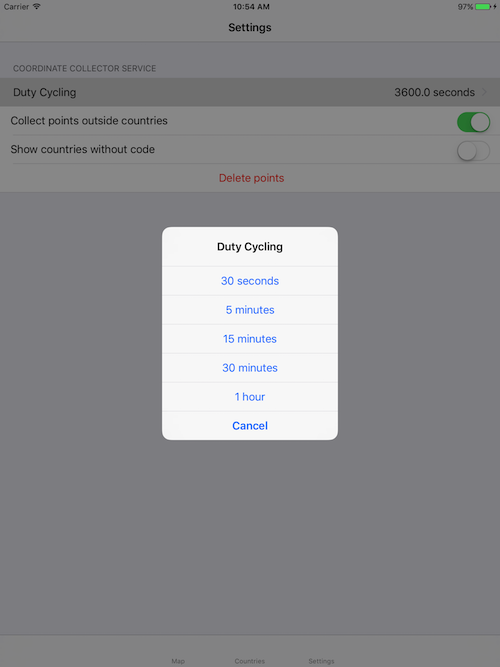
\includegraphics[width=0.4\textwidth]{images/duty_cycling.png}
	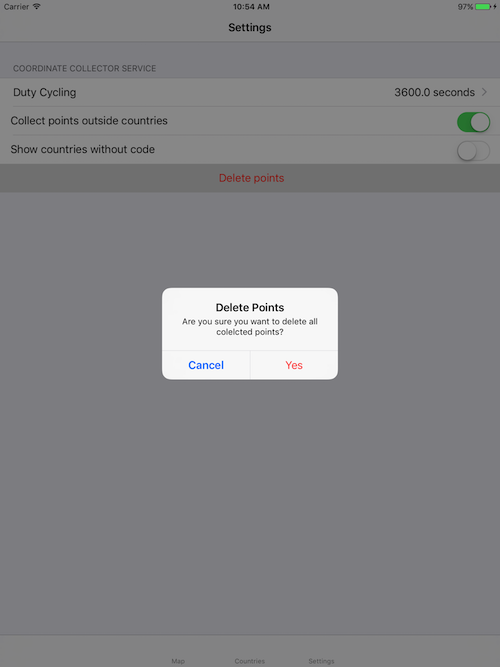
\includegraphics[width=0.4\textwidth]{images/point_deletion.png}
	\caption{Modifying the duty cycling schedule (left) and deleting points from the database (right).}
	\label{modification_of_settings}
	\end{center}
	\end{figure}

\section{Conclusions and future plans}
To summarize the project, the first version of the Scratch-Off Map application was developed for iOS devices as explained in the first chapter. Most of the features presented in Table \ref{feature-list} were developed: only feature \# 7 and \# 9 was not added due to their low priority and strong user interface oriented usage. These features can be added to the next version of the software. The rest of the features were more closely related to the contents of the Location Awareness course and therefore were ranked as higher priority and in the end are already parts of the application.

To support software quality, the test project includes 21 automated tests already. These ensure the correctness of the business logic and serve as validity-check during any future development. 

The main part of the business logic that is strongly related to the course is the duty cycling mechanism, the coordinate collection and the reverse-geocoding service. The first service was implemented in a manner that the code is reusable and can be ported to other applications. During the development of the other two services I had to study part of the MapKit API, which is a great tool for working with location data on the iOS platform. 

Future development may include the improvement of the $GeoCoder$ service as there is still a small room for improvement. As pointed out above, the number of requests to the reverse-geocoding service is limited and the application should embed a schedule to make the queries fluent and more reliable. Additionally, the application could be extended with features such as connection to and sharing results on social media, gamification, analysis of the collected points, colorizing the visited countries on the map and so on. 

\nocite{*}
\bibliographystyle{tktl}
\bibliography{lahteet}

\lastpage

\appendices

\pagestyle{empty}

%\internalappendix{1}{Model ABC}
%
%The appendices here are just models of the table of contents and the presentation. Each appendix 
%usually starts on its own page, with the name and number of the appendix at the top. Each appendix is paginated separately.
%
%In addition to complementing the main document, each appendix is also its own, independent entity. 
%This means that an appendix cannot be just an image or a piece of programming, but the appendix must explain its contents and meaning.

\end{document}